% Indicate the main file. Must go at the beginning of the file.
% !TEX root = ../main.tex

%----------------------------------------------------------------------------------------
% CHAPTER TEMPLATE
%----------------------------------------------------------------------------------------


\chapter{Methods} % Main chapter title

\label{Chapter3} % Change X to a consecutive number; for referencing this chapter elsewhere, use \ref{ChapterX}

%----------------------------------------------------------------------------------------
% SECTION 1
%----------------------------------------------------------------------------------------

\section{Training Data}



%-----------------------------------
% SUBSECTION 1
%-----------------------------------
\subsection{Data simulation}

The spectra were simulated with the Software Sessa v2.2.0 developed by Smekal et al. It uses binding energies from the NIST database and inelastic mean free paths (IMFPs) from various publications and simulations to calculate the spectra. Since version 2.2.0, it also accounts for energy dependence of the IMFP \cite{noauthor_nist_2010}.

As the probing depth of XPS is around 10 nanometers and the information diminishes rapidly after the first few nanometers, the thicknesses used for simulation of the top layer are n $\in$ [1, 2, 3, 4, 5] nm. A second simulation approach was to simulate slow transitions of elements such as seen in migration or alloying processes. As shown in \ref{fig:layers}

\begin{figure}
    \centering
    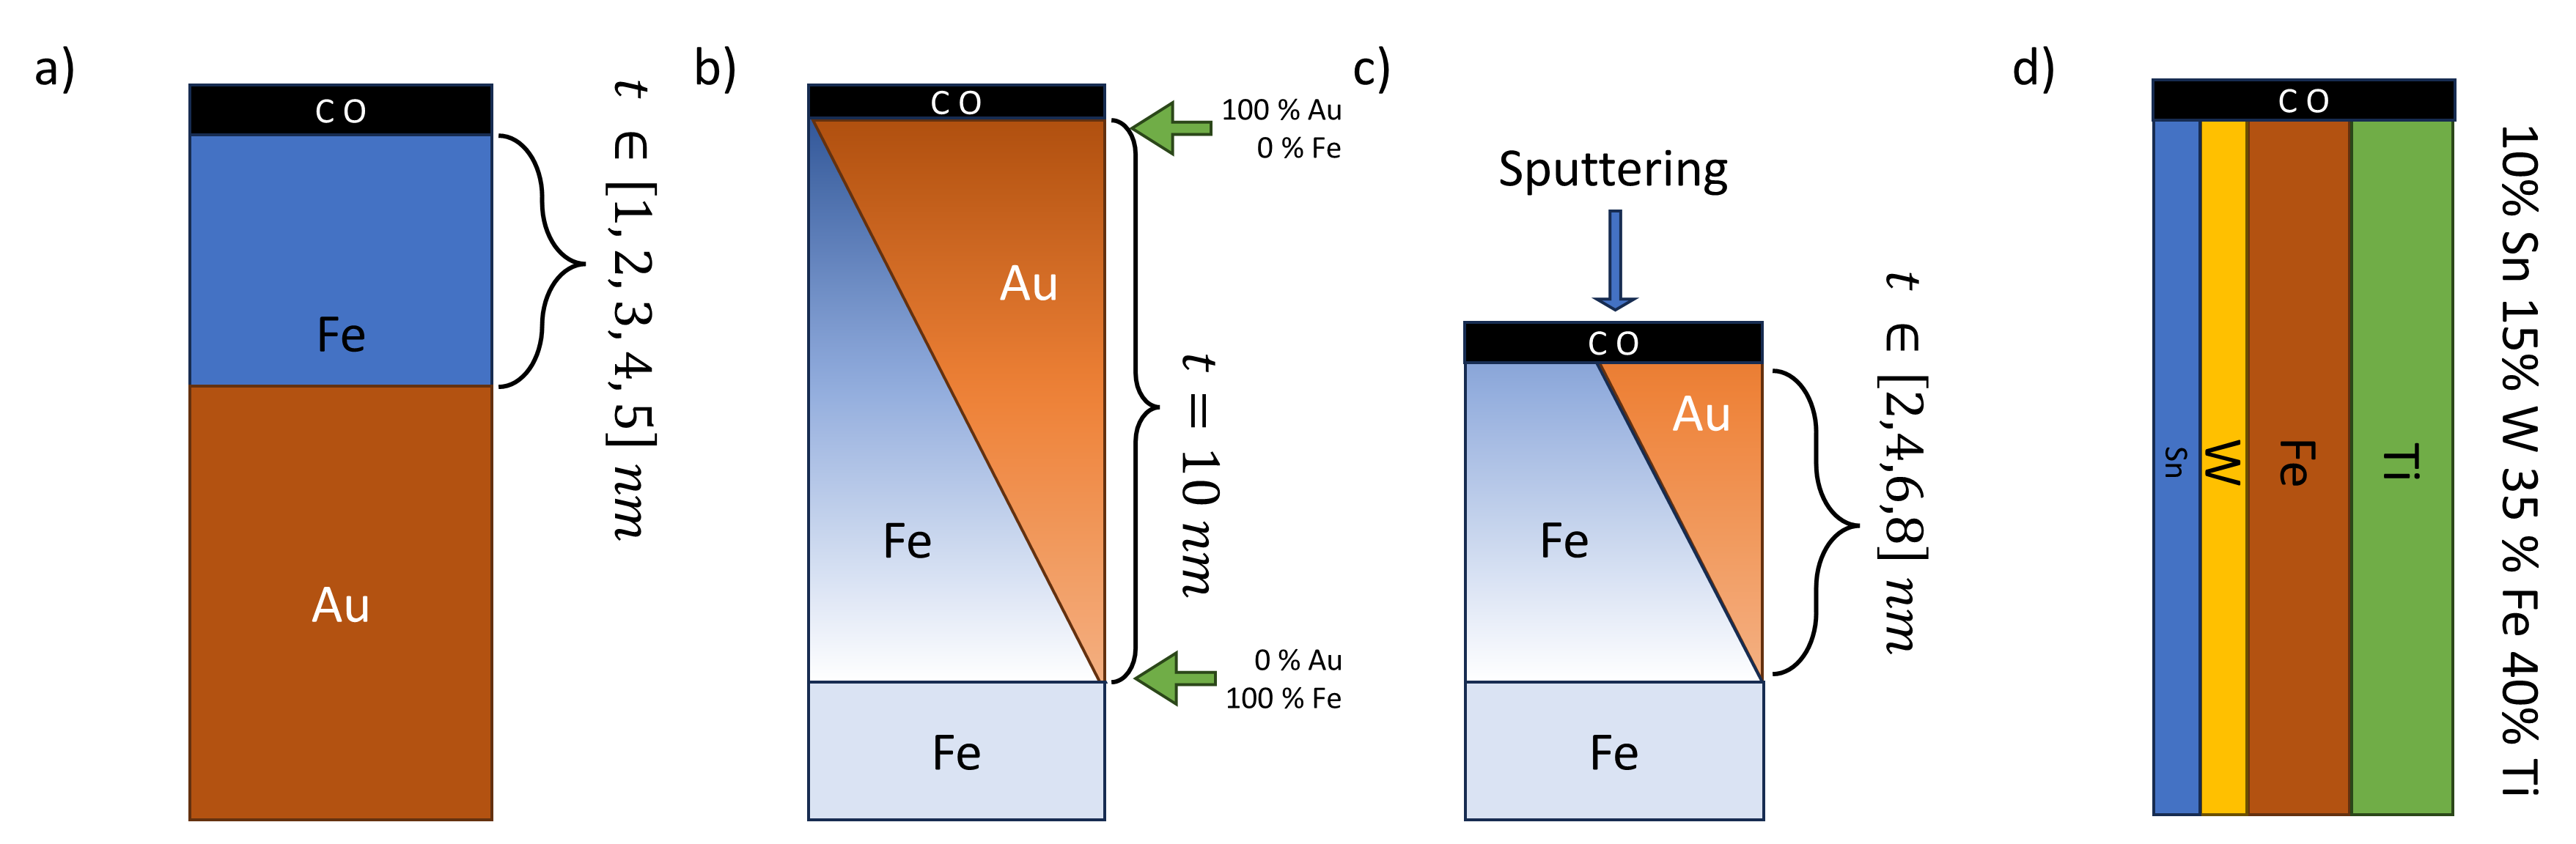
\includegraphics[scale=0.4]{Figures/layers.bmp}
    \caption{Simulation of layered systems}
    \label{fig:layers}
\end{figure}


The spectra simulated are using two components from all elements (n=81), thus 6561 permutations. With the 5 thicknesses, we obtain 32805 spectra for each experimental setup. To achieve a similar carbon and oxide content as experimental data (because of environmental influences), there is a carbon and oxide layer with thickness of triangular distribution (12-24, mode 15) Angstrom on top. 


Sessa v2.2.0, Python-Wrapper, Databases of Sessa, etc., X-Y-axis, carbon / oxygen layer, etc.

%-----------------------------------
% SUBSECTION 2
%-----------------------------------

\subsection{Data preprocessing}

Each spectra was max-normalized using equation \ref{eqn:normalize} 

\begin{equation}
    x' = \frac{x}{max(x)}
\label{eqn:normalize}
\end{equation}

%----------------------------------------------------------------------------------------
% SECTION 2
%----------------------------------------------------------------------------------------

\section{Test Data}

There are multiple sources for test-data of XPS-spectra. A main database was found on XPSlibrary, provided by TXL. Further, the XPSSurfA on CMSS Hub from the Australian University La Trobe contains more than 1700 spectra of which >100 survey spectra were used for the evaluation of the model.


\subsection{Data preprocessing}

As is typical for data acquired from laboratories, XPS data comes in various formats and measurement parameters. Apart from XPS-specific parameters, the resolution and the range mostly influence the evaluation of spectra with the deep-learning framework. Thus, an automated workflow for the spectra pre-processing is introduced to provide a valid entry point to the model.
Although most wide-survey spectra are measured with a comparable energy-range, it should be identical to the training data. Thus, any signal outside the specified binding energy range (0-1000 eV) is cut off and the discrete measurement points inside the range are interpolated or subsampled by using a uniformly distributed sampling method to match 1024 points.

The python module used to preprocess the data can be found in \ref{ApendixX}